\section{Supplementary Materials for the Experiments}

\subsection{Synthetic Settings}\label{app_synthetic}

\subsection{Image and Text Classification Settings}

Note: For text classification tasks, the source task training data size ranges from 500 to 1,500 and target task training data size is 1000; For ChestX-ray14, the training data size is 10,000.

\begin{figure}[!ht]
	\centering
	\begin{subfigure}[b]{0.33\textwidth}
		\centering
		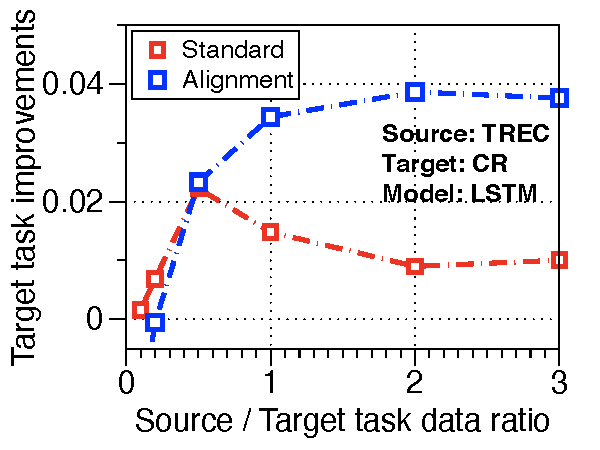
\includegraphics[width=0.975\textwidth]{figures/ratio_alignment_norm_trec_cr_lstm.pdf}
		\caption{Task pair TREC and CR}
	\end{subfigure}\hfill
		\begin{subfigure}[b]{0.33\textwidth}
		\centering
		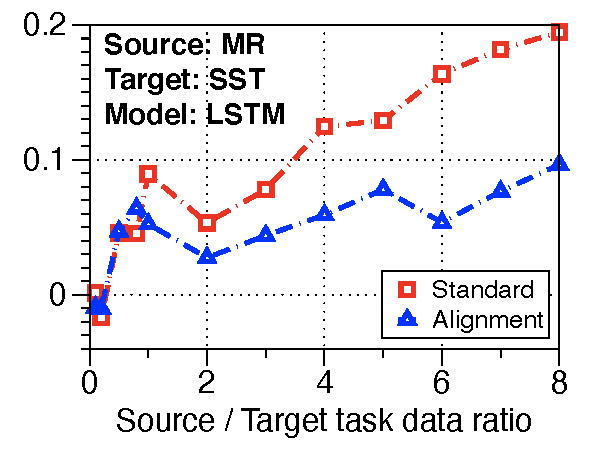
\includegraphics[width=0.975\textwidth]{figures/ratio_alignment_mr_sst_lstm.pdf}
		\caption{Task pair MR and SST}
	\end{subfigure}
	\caption{The performance of aligning task covariances depends on data size. As the ratio between source task data size and target task data size increases, the performance improvement from aligning task covariances increases.}
	\label{fig_covariate}
\end{figure}

